%!TEX root = Studienarbeit.tex

\documentclass[%
	pdftex,
	oneside,			% Einseitiger Druck.
	12pt,				% Schriftgroesse
	parskip=half,		% Halbe Zeile Abstand zwischen Absätzen.
	headheight = 12pt,	% Höhe der Kopfzeile
	headsepline,		% Linie nach Kopfzeile.
	footsepline,		% Linie vor Fusszeile.
	footheight = 16pt,	% Höhe der Fusszeile
	abstracton,		% Abstract Überschriften
	DIV=calc,		% Satzspiegel berechnen
	BCOR=8mm,		% Bindekorrektur links: 8mm
	headinclude=false,	% Kopfzeile nicht in den Satzspiegel einbeziehen
	footinclude=false,	% Fußzeile nicht in den Satzspiegel einbeziehen
	listof=totoc,		% Abbildungs-/ Tabellenverzeichnis im Inhaltsverzeichnis darstellen
	toc=bibliography,	% Literaturverzeichnis im Inhaltsverzeichnis darstellen
]{scrreprt}

% !TEX root =  arbeit.tex

\newcommand{\titel}{BLE HID Hardware-Erweiterungsmodul für Drohnenfernbedienungen}
\newcommand{\art}{Studienarbeit}
\newcommand{\autor}{Fabian Kuffer}
\newcommand{\studienbereich}{IT-Automotive}
\newcommand{\bearbeitungszeitraum}{4. Oktober 2022 - 8. Juni 2023}
\newcommand{\matrikelnr}{2044882}
\newcommand{\kurs}{TINF-20ITA}
\newcommand{\betreuer}{Prof. Dr. Karl Friedrich Gebhardt}
\newcommand{\datumAbgabe}{20. August 2022}
%!TEX root = Studienarbeit.tex

\usepackage{xstring}
\usepackage[utf8]{inputenc}
\usepackage[T1]{fontenc}
\usepackage{setspace}
\usepackage{longtable}

%bezeichnungen auf deutsch anpassen
\usepackage[english,ngerman]{babel}

\usepackage{makeidx}
\usepackage[margin=2.5cm,foot=1cm]{geometry}	% Seitenränder und Abstände
\usepackage[activate]{microtype} %Zeilenumbruch und mehr
%\usepackage[onehalfspacing]{setspace}
\usepackage[autostyle=true,german=quotes]{csquotes}
\usepackage{longtable}
\usepackage{enumitem}	% mehr Optionen bei Aufzählungen
\usepackage{graphicx}
\usepackage{pdfpages}   % zum Einbinden von PDFs
\usepackage{xcolor} 	% für HTML-Notation
\usepackage{float}
\usepackage{array}
\usepackage{calc}		% zum Rechnen (Bildtabelle in Deckblatt)
\usepackage[right]{eurosym}
\usepackage{wrapfig}
\usepackage{pgffor} % für automatische Kapiteldateieinbindung
\usepackage[perpage, hang, multiple, stable]{footmisc} % Fussnoten
\usepackage[printonlyused]{acronym} % falls gewünscht kann die Option footnote eingefügt werden, dann wird die Erklärung nicht inline sondern in einer Fußnote dargestellt
\usepackage{listings}

% Notizen. Einsatz mit \todo{Notiz} oder \todo[inline]{Notiz}. 
\usepackage[obeyFinal,backgroundcolor=yellow,linecolor=black]{todonotes}
% Alle Notizen ausblenden mit der Option "final" in \documentclass[...] oder durch das auskommentieren folgender Zeile
% \usepackage[disable]{todonotes}

% Literaturverweise
\usepackage[
	backend=biber,		% empfohlen. Falls biber Probleme macht: bibtex
	bibwarn=true,
	bibencoding=utf8,	% wenn .bib in utf8, sonst ascii
	sortlocale=de_DE,
	style=numeric,
]{biblatex}

% PDF Einstellungen
\usepackage[%
	pdftitle={\titel},
	pdfauthor={\autor},
	pdfsubject={\art},
	pdfcreator={pdflatex, LaTeX with KOMA-Script},
	pdfpagemode=UseOutlines, 		% Beim Oeffnen Inhaltsverzeichnis anzeigen
	pdfdisplaydoctitle=true, 		% Dokumenttitel statt Dateiname anzeigen.
	pdflang={de}, 			% Sprache des Dokuments.
]{hyperref}

% Workaround um Fehler in Hyperref, muss hier stehen bleiben
\usepackage{bookmark} %nur ein latex-Durchlauf für die Aktualisierung von Verzeichnissen nötig

%schriftart
\usepackage{lmodern}

%lorem ipsum generator
\usepackage{lipsum}

% (Farb-)einstellungen für die Links im PDF
\hypersetup{%
	colorlinks=true, 		% Aktivieren von farbigen Links im Dokument
	linkcolor={HTML}{00007A}, 	% Farbe festlegen
	citecolor={HTML}{00007A},
	filecolor={HTML}{00007A},
	menucolor={HTML}{00007A},
	urlcolor={HTML}{00007A},
	linktocpage=true, 		% Nicht der Text sondern die Seitenzahlen in Verzeichnissen klickbar
	bookmarksnumbered=true 	% Überschriftsnummerierung im PDF Inhalt anzeigen.
}

% Schriftart in Captions etwas kleiner
\addtokomafont{caption}{\small}


% Hurenkinder und Schusterjungen verhindern
% http://projekte.dante.de/DanteFAQ/Silbentrennung
\clubpenalty = 10000 % schließt Schusterjungen aus (Seitenumbruch nach der ersten Zeile eines neuen Absatzes)
\widowpenalty = 10000 % schließt Hurenkinder aus (die letzte Zeile eines Absatzes steht auf einer neuen Seite)
\displaywidowpenalty=10000

% Bildpfad
\graphicspath{{Bilder/}}

\begin{document}

    % Deckblatt
    \begin{spacing}{1}
        %!TEX root = arbeit.tex

\begin{titlepage}
	\enlargethispage{20mm}
	\begin{center}
		\vspace*{12mm}	{\LARGE\textbf \titel}\\
		\vspace*{12mm}	{\large\textbf \art}\\
		\vspace*{12mm}	{des Studiengangs \studienbereich}\\
		\vspace*{3mm}	{an der Dualen Hochschule Baden-Württemberg Stuttgart}\\
		\vspace*{12mm}	{von}\\
		\vspace*{3mm}		{\large\textbf \autor}\\
		\vspace*{12mm}	\today\\
	\end{center}
	\vfill
	\begin{spacing}{1.2}
	\begin{tabbing}
		mmmmmmmmmmmmmmmmmmmmmmmmmm		\= \kill
		\textbf{Bearbeitungszeitraum}	\>  \bearbeitungszeitraum\\
		\textbf{Matrikelnummer, Kurs}	\>  \matrikelnr, \kurs\\
		\textbf{Betreuer}				\>  \betreuer\\
	\end{tabbing}
	\end{spacing}
\end{titlepage}
    \end{spacing}
    \newpage

    \pagenumbering{Roman}

	% Erklärung
	%!TEX root = ../Studienarbeit.tex

\thispagestyle{empty}

\section*{Erklärung}
\vspace*{2em}

Ich versichere hiermit, dass ich meine {\art} mit dem Thema: {\itshape \titel } selbstständig verfasst und keine anderen als die angegebenen Quellen und Hilfsmittel benutzt habe. Ich versichere zudem, dass die eingereichte elektronische Fassung mit der gedruckten Fassung übereinstimmt. 

\vspace{3em}

Stuttgart, \today
\vspace{4em}

\rule{6cm}{0.4pt}\\
\autor
	\newpage

    % Abstract
	%!TEX root = ../Studienarbeit.tex

\pagestyle{empty}

\newenvironment{abstractpage}
  {\cleardoublepage\vspace*{\fill}\thispagestyle{empty}}
  {\vfill\cleardoublepage}
\newenvironment{abstractsection}[1]
  {\bigskip
   \begin{center}\bfseries#1\end{center}}
  {\par\bigskip}

\begin{abstractpage}
    \begin{abstractsection}{Kurzfassung}
        \todo[inline]{Kurzfassung}
    \end{abstractsection}

    \begin{abstractsection}{Abstract}
      \todo[inline]{Abstract}
    \end{abstractsection}
\end{abstractpage}
	\newpage

    \pagestyle{plain}		% nur Seitenzahlen im Fuß
	\RedeclareSectionCommand[beforeskip=20pt]{chapter} % stellt Abstand vor Kapitelüberschriften ein

	% Inhaltsverzeichnis
	\begin{spacing}{1.1}
		\begingroup
		
			% auskommentieren für Seitenzahlen unter Inhaltsverzeichnis
			\renewcommand*{\chapterpagestyle}{empty}
			\pagestyle{empty}
			
			
			\setcounter{tocdepth}{1}
			%für die Anzeige von Unterkapiteln im Inhaltsverzeichnis
			\setcounter{tocdepth}{2}
			
			\tableofcontents
			\clearpage
		\endgroup
	\end{spacing}
	\newpage

    % Abkürzungsverzeichnis
	\cleardoublepage
	%!TEX root = ../Studienarbeit.tex

\addchap{Abkürzungsverzeichnis}
%nur verwendete Akronyme werden letztlich im Abkürzungsverzeichnis des Dokuments angezeigt
%Verwendung: 
%		\ac{Abk.}   --> fügt die Abkürzung ein, beim ersten Aufruf wird zusätzlich automatisch die ausgeschriebene Version davor eingefügt bzw. in einer Fußnote (hierfür muss in header.tex \usepackage[printonlyused,footnote]{acronym} stehen) dargestellt
%		\acs{Abk.}   -->  fügt die Abkürzung ein
%		\acf{Abk.}   --> fügt die Abkürzung UND die Erklärung ein
%		\acl{Abk.}   --> fügt nur die Erklärung ein
%		\acp{Abk.}  --> gibt Plural aus (angefügtes 's'); das zusätzliche 'p' funktioniert auch bei obigen Befehlen
%	siehe auch: http://golatex.de/wiki/%5Cacronym
%	
\begin{acronym}[YTMMM]

    \acro{ADC}{Analog-Digital-Wandler}
    \acro{API}{application programming interface}
    \acro{ATT}{Attribute Protocol}
    \acro{BBR}{Bluetooth Basic Rate}
    \acro{BLE}{Bluetooth Low Energy}
    \acro{CE}{conformit\'e europ\'eenne}
    \acro{CID}{Kanalidentifizierer}
    \acro{CPU}{central processing unit}
    \acro{CRC}{Cyclic redundancy check}
    \acro{ESD}{Electro-Static-Discharge}
    \acro{ESP-IDF}{Espressif IoT Development Framework}
    \acro{evdev}{Event Device}
    \acro{FCC}{Federal Communications Commission}
    \acro{FIFO}{First In First Out}
    \acro{GAP}{Generic Access Profile}
    \acro{GATT}{Generic Attribute Profile}
    \acro{GPIO}{general purpose input/output}
    \acro{HCI}{Host Controller Interface}
    \acro{HID}{Human Interface Device}
    \acro{HOGP}{\acs{HID} over \acs{GATT} Profile}
    \acro{IC}{integrated circuit}
    \acro{IOCTL}{input output Control}
    \acro{ISM}{Industrial, Scientific and Medical}
    \acro{I2C}[I\textsuperscript{2}C]{inter integrated circuit}
    \acro{LDO}{Low-dropout regulator}
    \acro{LED}{light-emitting diode}
    \acro{LL}{Link Layer}
    \acro{L2CAP}{Logical Link Control and Adaption Protocol}
    \acro{MFi}{Made for iPhone/iPad/IPad}
    \acro{OLED}{organic light-emitting diode}
    \acro{PHY}{Physical Layer}
    \acro{PPM}{Puls-Positions-Modulation}
    \acro{RAM}{Random-access memory}
    \acro{RED}{Radio Equipment Directive}
    \acro{RPA}{Resolvable Private Address}
    \acro{SAR}{successive approximation}
    \acro{SDP}{Service Discovery Protocol}
    \acro{SIG}{Special Interest Group}
    \acro{SMP}{Security Manager Protocol}
    \acro{UART}{Universal Asynchronous Receiver Transmitter}
    \acro{UUID}{universal unique identifier}
    \acro{WLAN}{Wireless Local Area Network}
\end{acronym}

	% Abbildungsverzeichnis
	\cleardoublepage
	\listoffigures

	%Tabellenverzeichnis
	\cleardoublepage
	\listoftables

	% Quellcodeverzeichnis
	\cleardoublepage
	\lstlistoflistings
	\cleardoublepage

    \pagenumbering{arabic}
	
	\pagestyle{headings}		% Kolumnentitel im Kopf, Seitenzahlen im Fuß

	% Inhalt
	\foreach \i in {01,02,03,04,05,06,07,08,09,...,99} {%
		\edef\FileName{Kapitel/\i kapitel}%
			\IfFileExists{\FileName}{%
				\input{\FileName}
			}
			{%
				%file does not exist
			}
	}

	\clearpage

	% Literaturverzeichnis
	\cleardoublepage
	\printbibliography
	
	% sonstiger Anhang
	\clearpage
	\appendix
	% !TeX root = ../Studienarbeit.tex

\addchap{Anhang}
{\Large
\begin{enumerate}[label=\Alph*.]
	\item Schaltpläne
\end{enumerate}
}
\pagebreak
\section*{A.Schaltpläne}
\begin{figure}[htp]
    \centering
    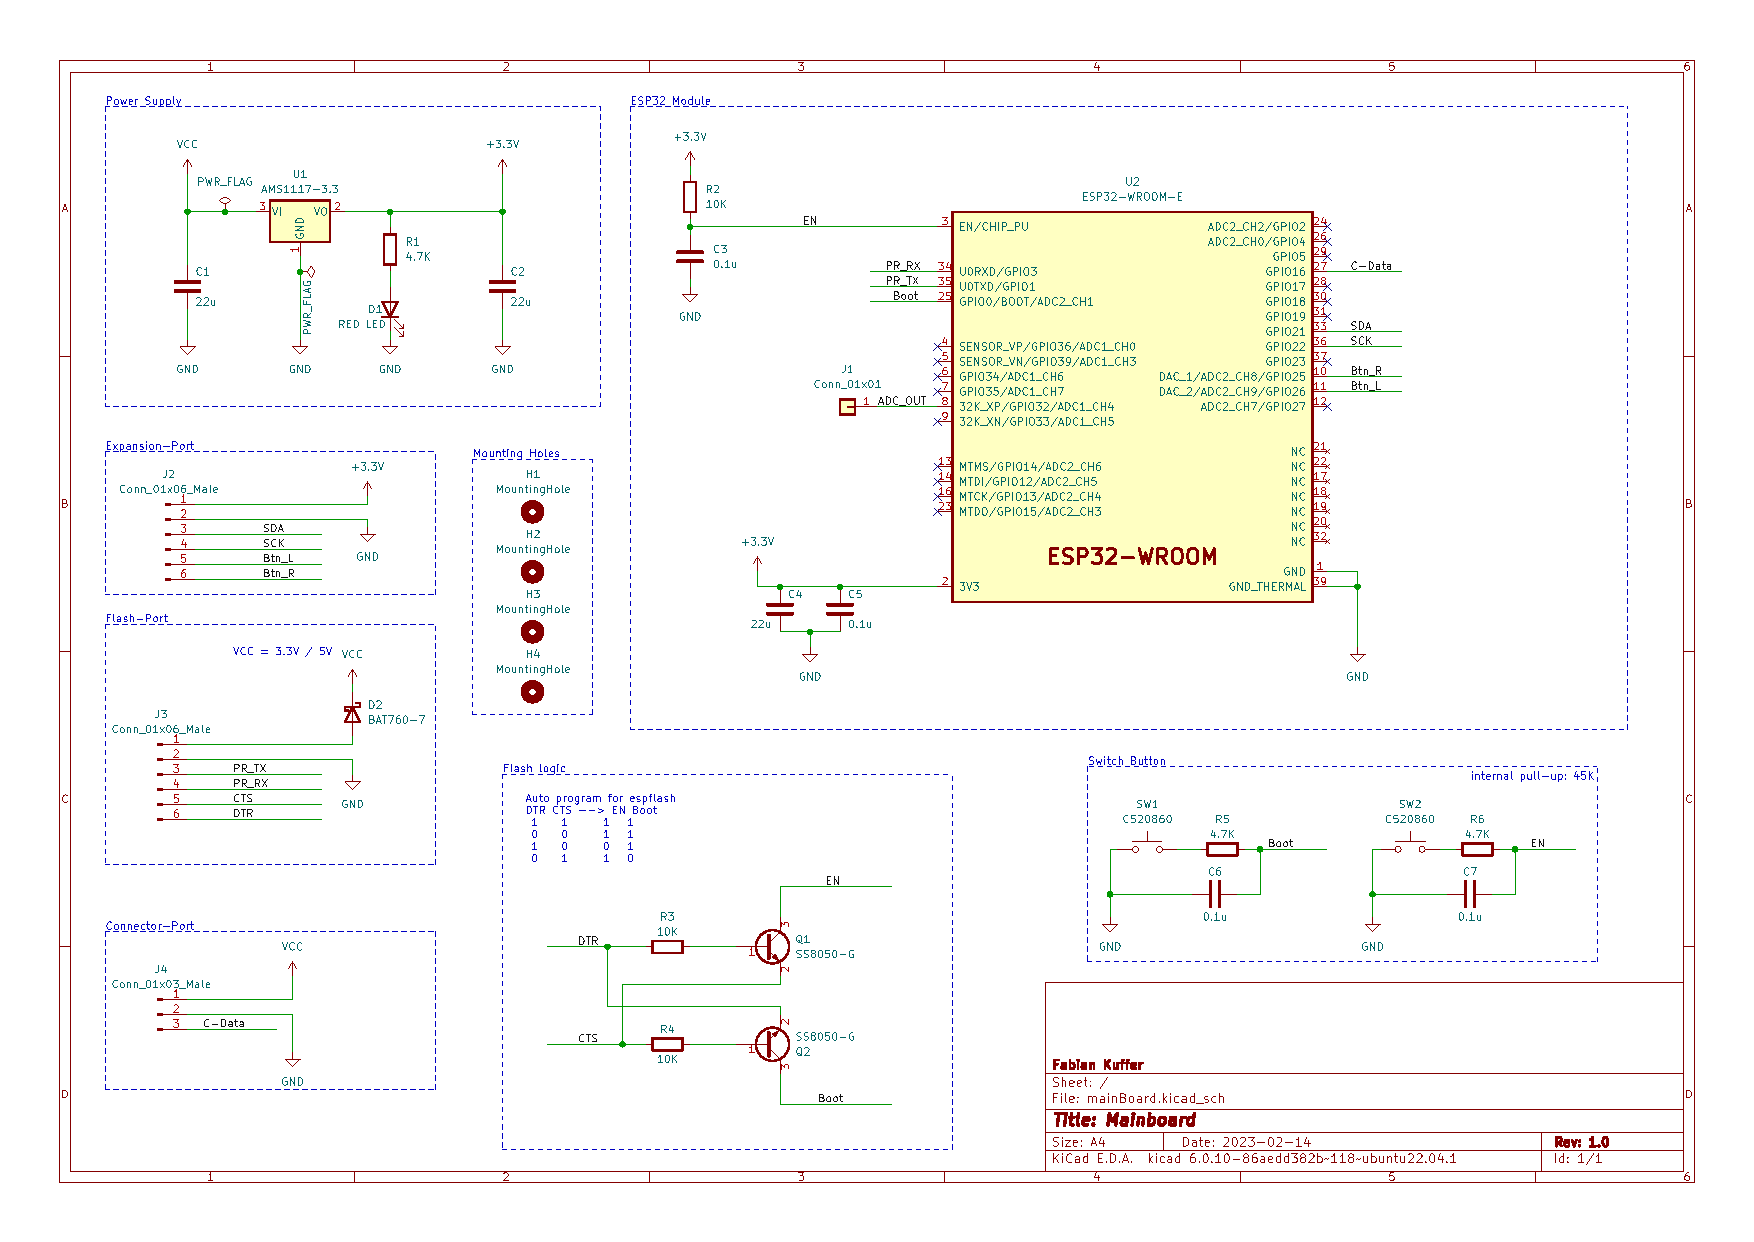
\includegraphics[width=1\textwidth]{../PDFs/mainBoard.pdf}
    \caption{Schaltplan der Hauptplatine}
    \label{fig:mainPCB}
\end{figure}

\begin{figure}[htp]
    \centering
    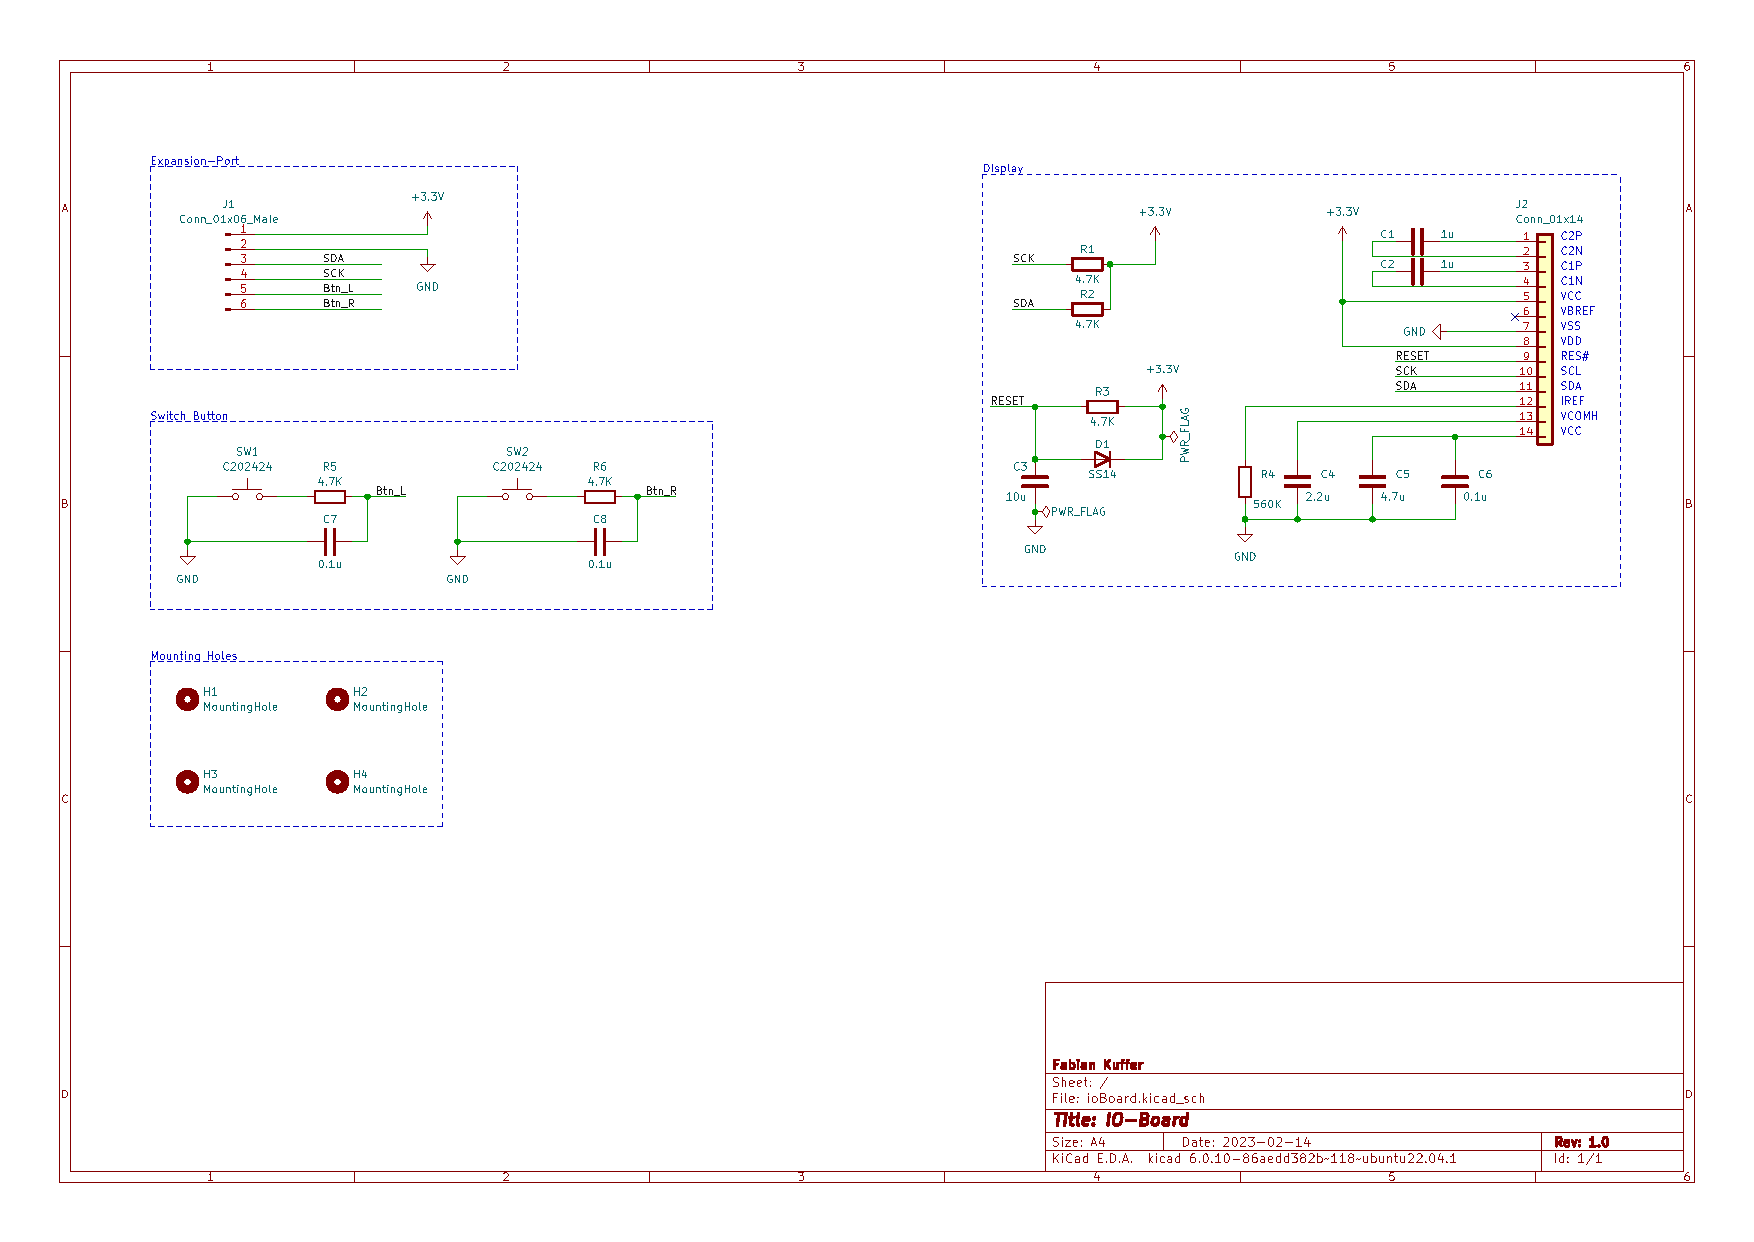
\includegraphics[width=1\textwidth]{../PDFs/ioBoard.pdf}
    \caption{Schaltplan für Ein- und Ausgabekomponenten}
    \label{fig:ioPCB}
\end{figure}

\begin{figure}[htp]
    \centering
    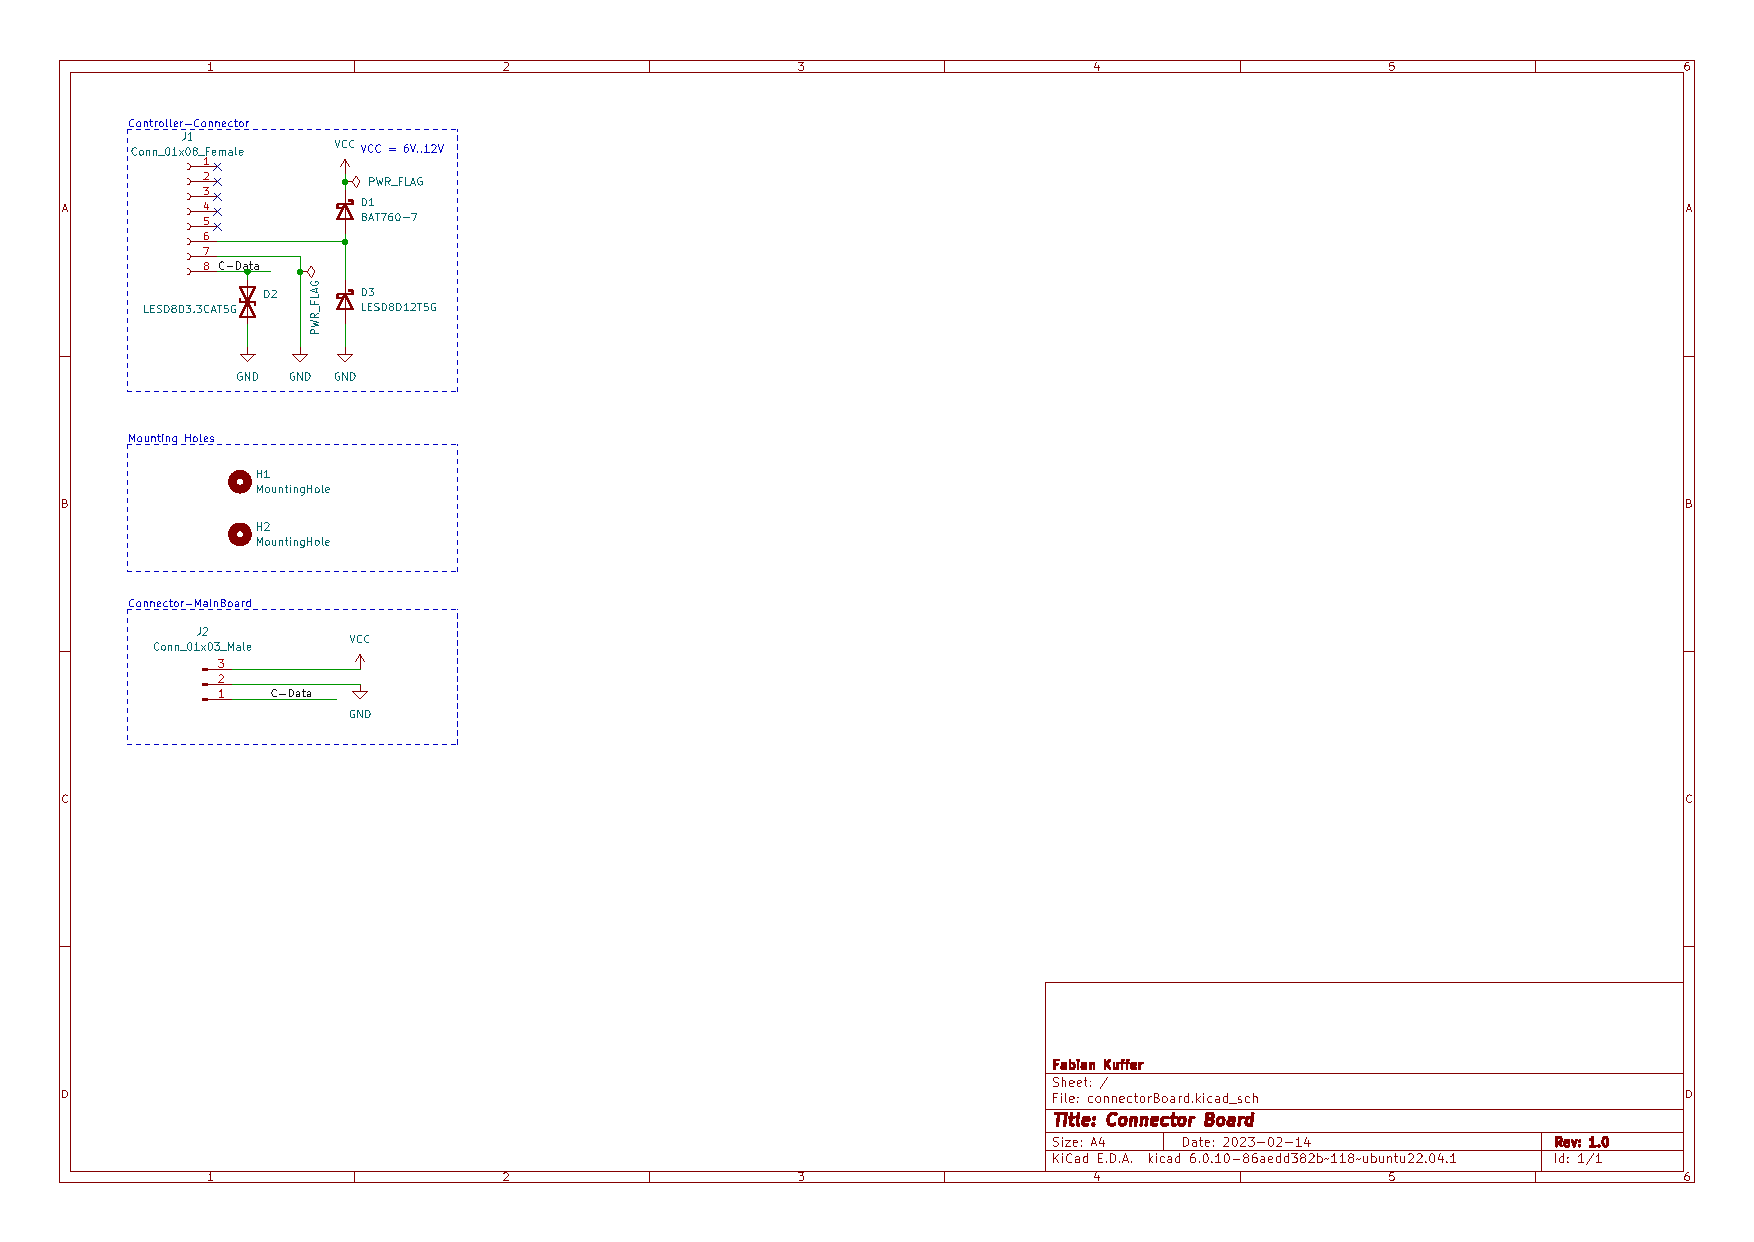
\includegraphics[width=1\textwidth]{../PDFs/connectorBoard.pdf}
    \caption{Schaltplan für die Verbindung zwischen Erweiterungsmodul und Multikopterfernsteuerung}
    \label{fig:connectorPCB}
\end{figure}
    
\end{document}